\section{Experiments}\label{sec:exp}
We aim to answer the following research questions:
\textbf{(1)} How well does our framework automatically formulate and synthesize manipulation behaviors (Sec.~\ref{sec:result})? 
\textbf{(2)} Can our system generalize to novel objects and manipulation strategies (Sec.~\ref{sec:generalization})?
\textbf{(3)} How do the individual components contribute to the failure cases of the system (Sec.~\ref{sec:error})?
We validate~\algabrvname on two real robot platforms: a wheeled single-arm platform, and a stationary dual-arm platform (Figure.~\ref{fig:viz}).
Additional implementation details can be found in Appendix, including keypoint proposal (\ref{app:proposal}), VLM querying (\ref{app:prompt}), point trackers (\ref{app:tracker}), sub-goal solver (\ref{app:subgoal}), and path solver (\ref{app:path}).





\subsection{\algabrvname for In-the-Wild and Bimanual Manipulation}\label{sec:result}

\begin{wrapfigure}{r}{0.38\textwidth}
\vspace{-1em}
  \centering
    \footnotesize
    \setlength\tabcolsep{2pt}
    \renewcommand{\arraystretch}{1.05}
    \begin{tabular}{@{}lcccc@{}}
        \toprule
         &  & \multicolumn{2}{c}{\textbf{\algabrvname}}\\
        \cmidrule(lr){3-4}
        \textbf{Task} & \textbf{VoxPoser} & Auto & Annot. \\
        \midrule
        \textbf{Mobile Arm}\\
        Pour Tea & 0/10 & 3/10 & 8/10  \\
        Recycle Can & 3/10 & 6/10 & 8/10  \\
        Stow Book & 0/10 & 3/10 & 6/10  \\ 
        Tape Box & 4/10 & 7/10 & 8/10  \\
        \midrule
        \textbf{Dual-Arm}\\
        Fold Garment  & 0/10 & 5/10 & 6/10  \\
        Pack Shoes & 0/10 & 3/10 & 5/10  \\
        Collab. Folding & 0/10 & 4/10 & 7/10  \\
        \midrule
        \textbf{Total (\%)} & 10.0\% & 44.3\% & 68.6\% \\
        \bottomrule
    \end{tabular}
    \vspace{0.1em}
    \captionof{table}{\small Success rate on wheeled single-arm and stationary bimanual platforms.}
    \label{tab:exps}
    \centering
    \footnotesize
    \setlength\tabcolsep{1.3pt}
    \renewcommand{\arraystretch}{1.05}
    \begin{tabular}{@{}lcccc@{}}
        \toprule
         &  & \multicolumn{2}{c}{\textbf{\algabrvname}}\\
        \cmidrule(lr){3-4}
        \textbf{Task (Dist.)} & \textbf{VoxPoser} & Auto & Annot. \\
        \midrule
        Pour Tea  & 0/10 & 2/10 & 4/10  \\
        Tape Box & 2/10 & 3/10 & 5/10  \\
        Collab. Folding & 0/10 & 3/10 & 5/10  \\
        \midrule
        \textbf{Total (\%)} & 6.7\% & 26.7\% & 46.7\% \\
        \bottomrule
    \end{tabular}
    \vspace{0.1em}
    \captionof{table}{\small Success rate under external disturbances across both robot platforms.}\label{tab:dist}
    \vspace{-0.8em}
    \begin{center}
    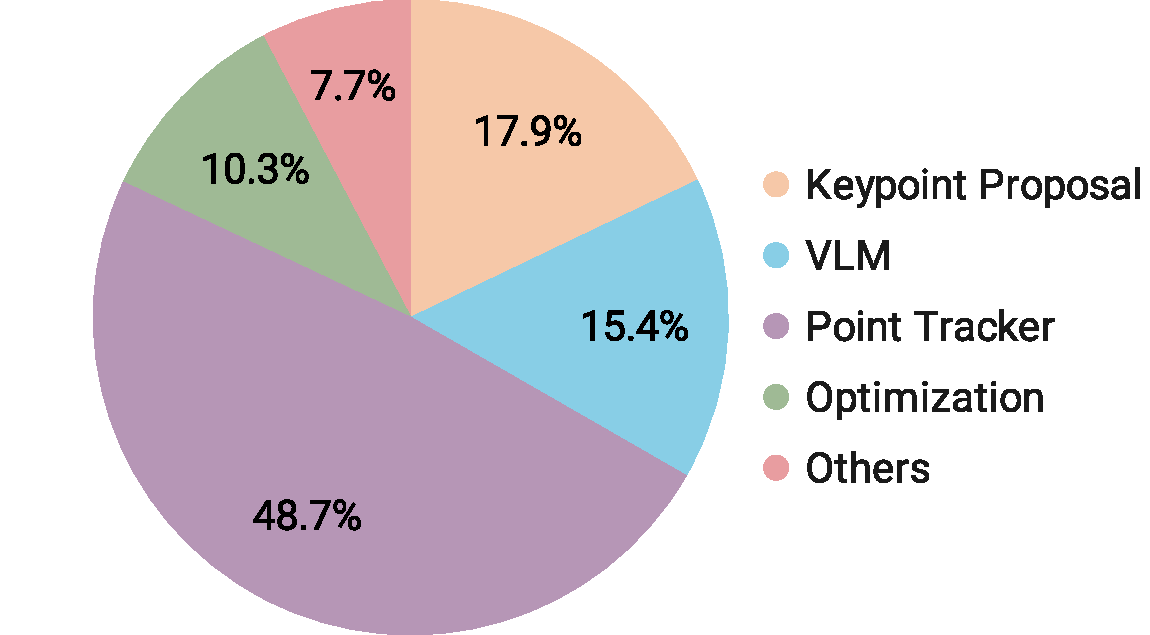
\includegraphics[width=0.7\linewidth]{media/error.pdf}
    \end{center}
    \vspace{-0.5em}
    \captionof{figure}{\small System error breakdown.}
    \label{fig:error}
    \vspace{-3.em}
\end{wrapfigure}

\textbf{Tasks.}
We purposefully select a set of tasks (shown in Fig.~\ref{fig:viz}) with the goal of examining the multi-stage (\textbf{m}), in-the-wild (\textbf{w}), bimanual (\textbf{b}), and reactive (\textbf{r}) behaviors of the system. The tasks and their features are \textit{Pour Tea} (\textbf{m}, \textbf{w}, \textbf{r}), \textit{Stow Book} (\textbf{w}), \textit{Recycle Can} (\textbf{w}), \textit{Tape Box} (\textbf{w}, \textbf{r}), \textit{Fold Garment} (\textbf{b}), \textit{Pack Shoes} (\textbf{b}), and \textit{Collaborative Folding} (\textbf{b}, \textbf{r}).
We further evaluate three of the tasks under external disturbances (denoted as ``Dist.'') by changing poses of task objects during execution.

\textbf{Metric and Baselines.} Each setting has 10 trials, in which object poses are randomized. Success rate is reported in Tab.~\ref{tab:exps}.
We compare to VoxPoser~\cite{huang2023voxposer} as a baseline.
We evaluate two variants of the system: ``Auto'' uses foundation models to automatically generate~\algabrvname, and ``Annotated (Annot.)'' uses human-annotated~\algabrvname.


\textbf{Results.}
Compared to baselines,~\algabrvname can effectively handle core challenges of each task.
For example, it can formulate correct temporal dependency in multi-stage tasks (e.g., spout needs to be aligned with the cup before pouring), leverage commonsense knowledge (e.g., coke cans should be recycled), and construct coordination behaviors in both bimanual settings (e.g., folding left sleeve and right sleeve simultaneously) and human-robot collaboration setting (e.g., folding a large blanket by aligning the four corners together with human).
Coupled with an optimization framework, it can also generate kinematically challenging behaviors in confined spaces in the \textit{Stow Book} task and find a feasible solution that densely fits two shoes within a small volume in the \textit{Pack Shoes} task.
Since the keypoints are tracked at a high frequency, the system can react to external disturbances and replan both within stage and across stages.
Despite promising results, we also identify several limitations which are discussed in Sec.~\ref{sec:conclusion}.



 



\subsection{Generalization in Manipulation Strategies}\label{sec:generalization}

\textbf{Tasks.}
We systematically evaluate how novel manipulation strategies can be formulated by focusing on a single task, garment folding, but with 8 unique categories of garments, each demanding a unique way of folding and requiring both geometrical and commonsense reasoning.
Evaluation is done on the bimanual platform, presenting additional challenges in bimanual coordination.


\textbf{Metric.}
We use GPT-4o with a prompt containing only generic instructions with no in-context examples.
``Strategy Success'' measures whether generated~\algabrvname is feasible, which tests both the keypoint proposal module and the VLM, and ``Execution Success'' measures system success rate given feasible strategies for each clothing. Each is measured with 10 trials.

\textbf{Results.}
Interestingly, we observe drastically different strategies across categories, many of which are aligned with how humans might fold each garment.
For example, it can recognize that two sleeves often are folded together, prior to fully folding the clothes.
In cases where using two arms is unnecessary, akin to how humans fold clothes, only one arm is being used.
However, we do observe that the VLM may miss certain steps to complete the folding as the operator expected, but we recognize that this is inherently an open-ended problem often based on one's preferences.




\begin{figure}[t]
    \centering
    \footnotesize
    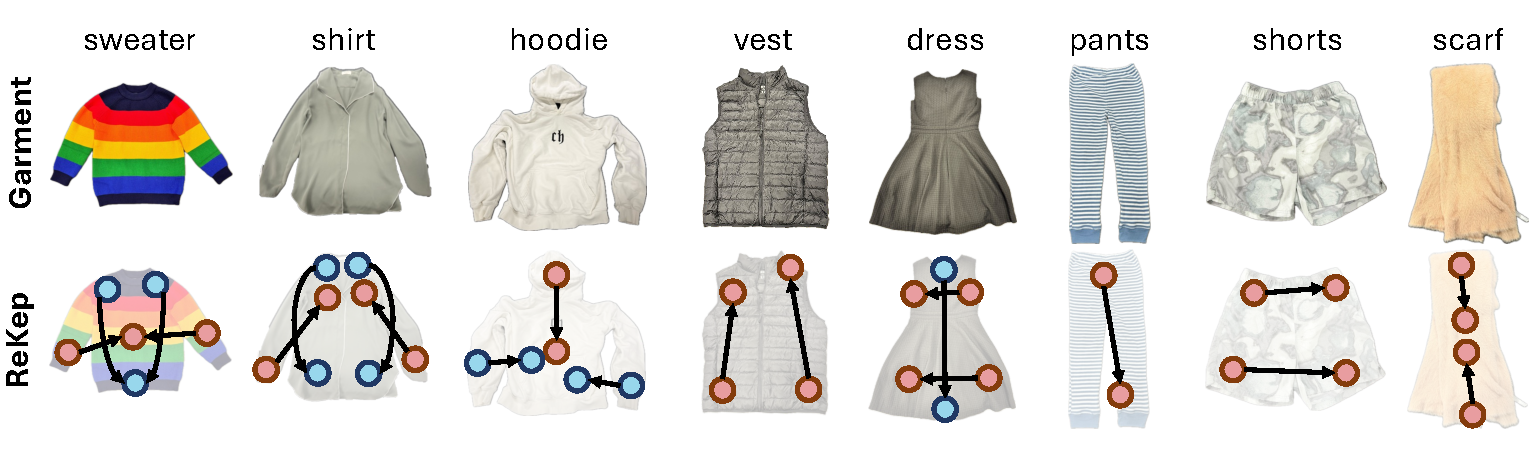
\includegraphics[width=0.85\linewidth]{media/generalization.pdf}
    \vspace{-1.2em}
    \begin{tabular}{@{}ccccccccccc@{}}
        \toprule
        \footnotesize
         & sweater & shirt & hoodie & vest & dress & pants & shorts & scarf & \textbf{Total}\\
        \midrule
        Strategy Success  & 6/10 & 4/10 & 4/10 & 6/10  & 3/10  & 7/10  & 7/10  & 5/10 & 52.5\% \\
        Execution Success & 6/10 & 5/10 & 6/10 & 9/10  & 7/10  & 8/10  & 9/10  & 9/10 & 73.8\% \\
        \bottomrule
    \end{tabular}
    \vspace{1.2em}
    \captionof{figure}{\small Novel \emph{bimanual} strategies of~\algabrvname for folding different categories of garments and their success rates. Since~\algabrvname in this task always associates two points at a time, two keypoints are connected by an arrow if they need to be aligned. The coloring of the keypoints denotes the order. In the sweater task, two sleeves are first folded simultaneously with two arms, and then the two arms grasp the crew neck to align to the bottom.}
    \label{tab:generalization}
    \vspace{-1.8em}
\end{figure}


\subsection{System Error Breakdown}\label{sec:error}


The modular design of the framework entails an advantage for analyzing system errors due to its interpretability.
In this section, we perform an empirical investigation by manually inspecting the failure cases of the experiments reported in Tab.~\ref{tab:exps}, which is then used to calculate the likelihood of a module causing an error while accounting for their temporal dependencies in the pipeline.
Results are reported in Fig.~\ref{fig:error}.
Among the different modules, the point tracker produces the largest portion of errors, as frequent and intermittent occlusion poses significant challenges for accurate tracking. %
Keypoint proposal and VLM also produce considerable portions of errors, where common cases include the proposal module missing certain keypoints and the VLM referring to incorrect keypoints.
The optimization module, on the other hand, does not contribute as much to the failures despite given limited time budget, since there often exist many possible solutions for each problem.
Other modules, such as segmentation, 3D reconstruction, and low-level controller, also contribute to some failure cases, but they are relatively insignificant compared to other modules.




